\subsubsection{Fundamento y Motivación}

El sistema mecánico del robot presenta holguras acumulativas que generan errores de posicionamiento de hasta ±5 milímetros respecto a la posición comandada. Estos errores resultan incompatibles con los requerimientos de precisión para las operaciones de cosecha, que exigen tolerancias inferiores a ±2 milímetros. Para compensar estas desviaciones se implementó un sistema de corrección visual basado en la detección de marcadores de referencia.

Los marcadores consisten en cintas adhesivas negras de 18 milímetros de ancho adheridas sobre la superficie de los tubos de PVC blanco del sistema hidropónico. Esta configuración proporciona un contraste óptico superior a 0.85 entre el elemento oscuro y el fondo claro, facilitando su detección mediante técnicas de procesamiento de imágenes. La selección de cintas adhesivas como elemento de marcado se fundamentó en su bajo costo de implementación (inferior a 5 dólares estadounidenses por metro lineal), su robustez ante las condiciones de humedad y temperatura del invernadero, y la facilidad de instalación sin modificaciones estructurales del sistema.

Las cintas se disponen en dos orientaciones: cintas horizontales que proporcionan referencia para corrección en el eje vertical, y cintas verticales que proporcionan referencia para corrección en el eje horizontal. Esta configuración dual permite la corrección independiente en ambos ejes de movimiento del robot.

\begin{figure}[h]
\centering
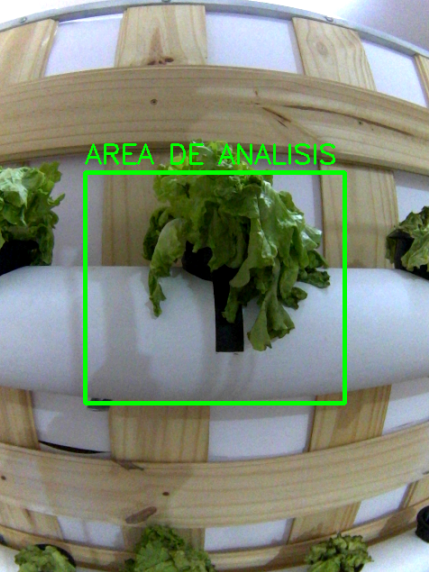
\includegraphics[width=0.75\textwidth]{imagenes/configuracion_cintas_referencia.png}
\caption{Disposición de cintas de referencia horizontal y vertical en el sistema hidropónico}
\label{fig:configuracion_cintas}
\end{figure}
